\section{Introduction}
L'unité PR202 s'inscrit dans la continuité de l'unité EL202. Ce projet nous demande de réaliser un jeu vidéo en VHDL jouable sur un écran VGA. Les objectifs sont nombreux. Techniquement, il nous permet d'améliorer notre connaissance du VHDL, de comprendre les bases de l'utilisation du VGA et de l'interfacage d'autre périphériques. Il nous introduit également aux protocoles liés au matériel. Ce projet est également l'occasion pour nous de perfectionner notre connaissance de la gestion de projet et d'avoir une autre expérience de la division du travail.\\

Notre trinôme a choisi de réaliser un PONG. Ce jeu vidéo développé par Atari en 1972 est le jeu qui a lancé l'industrialisation du jeu vidéo. Initialement sorti sous la forme d'une borne d'arcade, il donne vite naissance à une console dédiée \cite{cite:pong}.\\

\begin{figure}[h!]
	\centering
	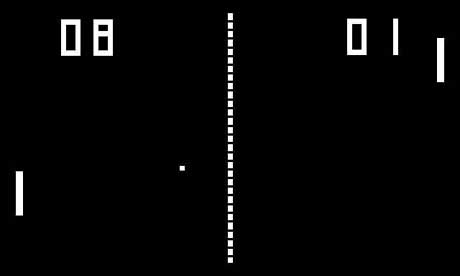
\includegraphics[scale=0.75]{images/pong.jpg}
	\caption{Capture d'écran de PONG (1972)}
	\label{fig:pong}
\end{figure}

\newpage
